\documentclass[11pt]{charter}

% El títulos de la memoria, se usa en la carátula y se puede usar el cualquier lugar del documento con el comando \ttitle
\titulo{Filtro de Kalman de Rango/Corrimiento Doppler para Sistema de Navegación} 

% Nombre del posgrado, se usa en la carátula y se puede usar el cualquier lugar del documento con el comando \degreename
\posgrado{Carrera de Especialización en Sistemas Embebidos} 
%\posgrado{Carrera de Especialización en Internet de las Cosas} 
%\posgrado{Carrera de Especialización en Intelegencia Artificial}
%\posgrado{Maestría en Sistemas Embebidos} 
%\posgrado{Maestría en Internet de las cosas}

% Tu nombre, se puede usar el cualquier lugar del documento con el comando \authorname
\autor{Alejandro Moreno} 

% El nombre del director y co-director, se puede usar el cualquier lugar del documento con el comando \supname y \cosupname y \pertesupname y \pertecosupname
\director{Dr. Ing. Juan Ignacio Giribet}
\pertenenciaDirector{FIUBA} 
% FIXME:NO IMPLEMENTADO EL CODIRECTOR ni su pertenencia
\codirector{} % si queda vacio no se deberíá incluir 
\pertenenciaCoDirector{}

% Nombre del cliente, quien va a aprobar los resultados del proyecto, se puede usar con el comando \clientename y \empclientename
\cliente{Mg. Ing. Manuel Francisco Díaz Ramos}
\empresaCliente{Satellogic S.A.}

% Nombre y pertenencia de los jurados, se pueden usar el cualquier lugar del documento con el comando \jurunoname, \jurdosname y \jurtresname y \perteunoname, \pertedosname y \pertetresname.
\juradoUno{Nombre y Apellido (1)}
\pertenenciaJurUno{pertenencia (1)} 
\juradoDos{Nombre y Apellido (2)}
\pertenenciaJurDos{pertenencia (2)}
\juradoTres{Nombre y Apellido (3)}
\pertenenciaJurTres{pertenencia (3)}
 
\fechaINICIO{22 de junio de 2020}		%Fecha de inicio de la cursada de GdP \fechaInicioName
\fechaFINALPlanificacion{22 de Agosto de 2020} 	%Fecha de final de cursada de GdP
\fechaFINALTrabajo{22 de Julio de 2021}		%Fecha de defensa pública del trabajo final

\newcolumntype{L}[1]{>{\raggedright\let\newline\\\arraybackslash\hspace{0pt}}m{#1}}
\newcolumntype{C}[1]{>{\centering\let\newline\\\arraybackslash\hspace{0pt}}m{#1}}
\newcolumntype{R}[1]{>{\raggedleft\let\newline\\\arraybackslash\hspace{0pt}}m{#1}}

\begin{document}

\maketitle
\thispagestyle{empty}
\pagebreak


\thispagestyle{empty}
{\setlength{\parskip}{0pt}
\tableofcontents{}
}
\pagebreak


\section{Registros de cambios}
\label{sec:registro}


\begin{table}[ht]
\label{tab:registro}
\centering

\begin{tabularx}{\linewidth}{@{}|c|X|c|@{}}
\hline
\rowcolor[HTML]{C0C0C0} 
Revisión & \multicolumn{1}{c|}{\cellcolor[HTML]{C0C0C0}Detalles de los cambios realizados} & Fecha      \\ \hline
1.0      & Creación del documento                                                          & 10/07/2020 \\ \hline
1.1      & Redacción del punto 6 - 12                                                      & 27/07/2020 \\ \hline
%1.1      & Ejemplo de un texto muy largo que debiera ocupar más de una línea para que tengan de ejemplo                                                                                																						   & dd/mm/aaaa \\ \hline
%1.2      & Otro ejemplo \newline
%		   Con texto partido \newline
%		   En varias líneas \newline
%		   A propósito                                                                     & dd/mm/aaaa \\ \hline
\end{tabularx}
\end{table}

\pagebreak



\section{Acta de Constitución del Proyecto}
\label{sec:acta}

\begin{flushright}
Buenos Aires, \fechaInicioName
\end{flushright}

\vspace{2cm}

Por medio de la presente se acuerda con el Ing. \authorname\hspace{1px} que su Trabajo Final de la \degreename\hspace{1px} se titulará ``\ttitle'', consistirá esencialmente en el prototipo preliminar de un Sistema de Navegación satelital para órbita terrestre baja, basado en un Filtro de Kalman que utilice el modelo cinemático orbital para la actualización temporal y los observables del GNSS para la actualización de las mediciones. Asimismo, contemplará el análisis comparativo de la solución propuesta con la actualmente adoptada por el cliente. El trabajo tendrá un presupuesto preliminar estimado de 600 hs de trabajo y una retribución económica a ser discutida con el cliente según los resultados obtenidos, con fecha de inicio \fechaInicioName\hspace{1px} y fecha de presentación pública \fechaFinalName.

Se adjunta a esta acta la planificación inicial.

\vfill

% Esta parte se construye sola con la información que hayan cargado en el preámbulo del documento y no debe modificarla
\begin{table}[ht]
\centering
\begin{tabular}{ccc}
\begin{tabular}[c]{@{}c@{}}Ariel Lutenberg \\ Director posgrado FIUBA\end{tabular} &  & \begin{tabular}[c]{@{}c@{}}\clientename \\ \empclientename \end{tabular} \vspace{2.5cm} \\ 
\multicolumn{3}{c}{\begin{tabular}[c]{@{}c@{}} \supname \\ Director del Trabajo Final\end{tabular}} \vspace{2.5cm} \\
\begin{tabular}[c]{@{}c@{}}\jurunoname \\ Jurado del Trabajo Final\end{tabular}     &  & \begin{tabular}[c]{@{}c@{}}\jurdosname\\ Jurado del Trabajo Final\end{tabular}  \vspace{2.5cm}  \\
\multicolumn{3}{c}{\begin{tabular}[c]{@{}c@{}} \jurtresname\\ Jurado del Trabajo Final\end{tabular}} \vspace{.5cm}                                                                     
\end{tabular}
\end{table}




\section{Descripción técnica-conceptual del Proyecto a realizar}
\label{sec:descripcion}

En las aplicaciones aeroespaciales resulta indispensable disponer de un sistema que permita estimar las variables que caracterizan al sistema bajo estudio. Por ejemplo, estimar la posición y velocidad con precisión y exactitud resultan de suma importancia y para lograrlo es necesario diseñar un sistema de navegación que contemple complejas interacciones entre sensores, cinemática y dinámica del sistema. En particular, una de las alternativas más ampliamente adoptadas para abordar el problema de estimación planteado es el uso de un Filtro de Kalman. 

En lo que respecta al presente trabajo se propone diseñar una solución basada en el mencionado Filtro de Kalman en alguna de sus variantes más conocidas: Kalman Linealizado, Kalman Extendido o Kalman Descentrado. Asimismo, dado que la utilización del estimador es para ser montado sobre un satélite, sabiendo que el mismo opera siguiendo una trayectoria predefinida desde su etapa de diseño, se opta por un modelo de actualización de estados basado en la dinámica orbital correspondiente a la aplicación en que será utilizada por el cliente, es decir órbita terreste baja. No obstante, este proyecto se destaca especialmente por incorporar una etapa de actualización de mediciones basada en los observables (pseudo-rango y corrimiento doppler) del receptor GNSS a una frecuencia de 1Hz. Esto lo diferencia de implementaciones más usuales basadas en datos ya procesados de posición y velocidad otorgadas por el GNSS.

Lo anteriormente mencionado resulta de sumo interés para el cliente puesto que su empresa se dedica a la comercialización de imágenes satelitales y para ello debe lidiar, ajustar y diseñar sus Sistemas de Control de Órbita y Actitud (AOCS) para conseguir las mejores prestaciones. Al mismo tiempo, dada la proyección de crecimiento de la flota de satélites que pretende administrar en los años venideros, se encuentra ventajoso explorar opciones alternativas a las actualmente utilizadas por la compañía para los sistemas de navegación puesto que la robustez y/o costos de fabricación podrían verse notoriamente beneficiados.

En la Figura~\ref{fig:diagBloques} se presenta el diagrama en bloques del sistema. Se puede apreciar que el sistema es sencillo de entender lo que lo convierte en un buen modelo abstracto del problema a solucionar.

\vspace{25px}

\begin{figure}[htpb]
\centering 
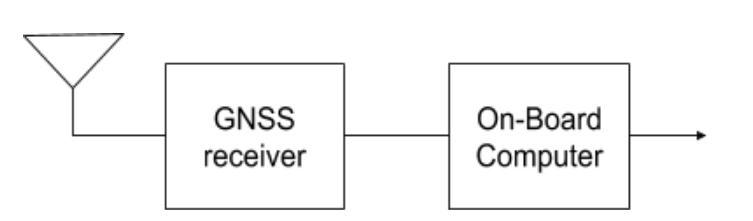
\includegraphics[width=.7\textwidth]{./Figuras/diagBloques.png}
\caption{Diagrama en bloques del sistema}
\label{fig:diagBloques}
\end{figure}

\vspace{25px}


\section{Identificación y análisis de los interesados}
\label{sec:interesados}

\begin{table}[H]
%\caption{Identificación de los interesados}
%\label{tab:interesados}
\begin{tabularx}{\linewidth}{@{}|l|X|X|l|@{}}
\hline
\rowcolor[HTML]{C0C0C0} 
Rol           & Nombre y Apellido & Organización 	& Puesto 	\\ \hline
Auspiciante   & \clientename      &\empclientename	& Satellite Systems Bus Team Leader \\ \hline
Cliente       & \clientename      &\empclientename	& Satellite Systems Bus Team Leader \\ \hline
Impulsor      & -                 & -             	& -      	\\ \hline
Responsable   & \authorname       & FIUBA        	& Alumno 	\\ \hline
Colaboradores &  -                & -             	& -      	\\ \hline
Orientador    & \supname	      		& \pertesupname & Director	Trabajo final \\ \hline
Equipo        & -						& -            	& -      	\\ \hline
Opositores    & -                 & -             	& -      	\\ \hline
Usuario final & Satellogic S.A.   & -             	& -      	\\ \hline
\end{tabularx}
\end{table}

\begin{itemize}
\item \textbf{Cliente:} es un experto en sistemas de Navegación, Control y Guiado. Amplia experiencia en la industria y formación académica profunda. Necesita que el proyecto se lleve adelante sin demasiada intervención por su parte porque su agenda está muy apretada. No contactar por nimiedades.
\item \textbf{Orientador:} es un experto en temas de Navegación, Control y Guiado. Amplia experiencia en proyectos de la industria aeroespacial y larga trayectoria académica. Es una persona conocida y de confianza pero tiene muchas obligaciones. En tal sentido, presentarle soluciones para que él las evalúe pero no pedirle intervención continuamente.
\end{itemize}


\section{1. Propósito del proyecto}
\label{sec:proposito}

El propósito del proyecto es realizar una prueba de concepto de un filtro de Kalman para un sistema de navegación integrado satelital. La entrada del filtro serán mediciones dadas por un receptor GNSS en forma de pseudo-rango y corrimiento doppler a 1 Hz y la salida serán estimaciones de posición-velocidad en tiempo real.

\section{2. Alcance del proyecto}
\label{sec:alcance}

El proyecto incluye los siguientes puntos: 

\begin{itemize}
\item Diseño de una biblioteca modular en C++ que permita parsear los mensajes con observaciones crudas de los observables del receptor GNSS.
\item Diseño de una biblioteca modular en C++ que permita convertir las observaciones de pseudo-rango/corrimiento Doppler en posición/velocidad ECEF-WGS84.
\item Diseño de una biblioteca modular en C++ con un Filtro de Kalman que permita tomar los datos parseados por el software desarrollado en el punto 1 para estimar la posición/velocidad ECEF-WGS84 en tiempo real.
\item Diseño de una biblioteca modular en C++ con un Filtro de Kalman que permita tomar los datos convertidos por el software desarrollado en el punto 2 para estimar la posición/velocidad ECEF-WGS84 en tiempo real.
\item Caracterizar y comparar el error de estimación realizando un análisis de covarianza y residuos para ambos filtros.
\end{itemize}

El presente proyecto no incluye el diseño ni la implementación del hardware necesario para el sistema de navegación diseñado. Quedando sujeto a la disponibilidad del cliente y del Ing. \authorname{} realizar pruebas con un receptor GNSS utilizado como hardware de vuelo y un simulador de constelación.

\section{3. Supuestos del proyecto}
\label{sec:supuestos}

Para el desarrollo del presente proyecto se supone que: 

\begin{itemize}
\item Se dispondrá de un archivo con los datos crudos de los observables del receptor GNSS y documentación del protocolo propietario que permita parsearlos.
\item Se dispondrá de la información relacionada a la performance del estimador que el cliente utiliza actualmente para poder hacer una análisis comparativo con la solución que surja del presente trabajo.
\item Se podrá contar con la ayuda de un experto en la materia para sortear las dificultades técnicas que surjan.
\item El contrato de confidencialidad celebrado entre el Laboratorio de Sistemas Embebidos (LSE) y el cliente no generá inconvenientes para consultar dudas o expertos en temas genéricos relacionados a los aspectos teóricos necesarios para arribar a una solución que satisfaga las necesidades del cliente.
\item La placa EDU-CIAA permitirá ejecutar el algoritmo suficientemente rápido y con suficiente precisión en los cálculos como para que el sistema de navegación funcione en tiempo real.
\item No se requerirá la certificación del sistema de navegación diseñado.
\item No ocurrirán eventos fortuitos ni de fuerza mayor que limiten la cantidad de horas semanales asignadas a este proyecto. 
\item En caso de optar por hacer las pruebas con el hardware y el simulador de constelaciones, se contará con toda la documentación necesaria para poder trabajar con el receptor GNSS y, al mismo tiempo, el cliente suministrará todos los materiales necesarios para su implementación, así como los equipos pertinentes para llevar adelante los testeos.
\end{itemize}


\section{4. Requerimientos}
\label{sec:requerimientos}

\begin{enumerate}
\item Requerimientos de documentación
	\begin{enumerate}
	\item Memoria Técnica con la documentación de ingeniería detallada.
	\item Bibliotecas de software adecuadamente documentada utilizando Doxygen.
	\item Documento que registre el avance del proyecto. Se realiza una vez siguiendo el cronograma que se establece en la Sección~\ref{sec:gantt}.
	\item Documento que registre la planificación inicial del proyecto. Se realiza una vez al comienzo del trabajo.
	\end{enumerate}
\item Requerimientos de la implementación del software:
	\begin{enumerate}
	\item Grupo de requerimientos asociados con la metodología de desarrollo:
		\begin{enumerate}
		\item Utilizar un sistema de control de versiones con repositorios on-line.
		\item Programar en lenguaje C++.
		\end{enumerate}
	\item Grupo de requerimientos asociados con los sensores:
		\begin{enumerate}
		\item Se encuestarán los observables del receptor GNSS (pseudo-rango y corrimiento doppler) cada 1 segundo. Encuesta tomada del archivo con los datos crudos.
		\end{enumerate}
	\item Grupo de requerimientos del Filtro de Kalman:
		\begin{enumerate}
		\item Utilizar alguna de las variantes tradicionales para estimar el vector de estados de un sistema no lineal: \textit{Linearized Kalman}, \textit{Extended Kalman} o \textit{Uncentered Kalman}.
		\item Utilizar un modelo de actualización de estados basado en el modelo astro-dinámico que caracteriza la mecánica orbital de los satélites de órbita terrestre baja.
		\item Utilizar un modelo de actualización de mediciones basado en la utilización del pseudo-rango y el corrimiento doppler cada 1 segundo.
		\end{enumerate}
	\end{enumerate}
\end{enumerate}

\section{Historias de usuarios (\textit{Product backlog})}
\label{sec:backlog}

\begin{consigna}{red}
En esta sección se deben incluir las historias de usuarios y su ponderación (history points). Recordar que las historias de usuarios son descripciones cortas y simples de una característica contada desde la perspectiva de la persona que desea la nueva capacidad, generalmente un usuario o cliente del sistema. La ponderación es un número entero que representa el tamaño de la historia comparada con otras historias de similar tipo.
\end{consigna}

\section{5. Entregables principales del proyecto}
\label{sec:entregables}

\begin{itemize}
\item Memoria Técnica.
\item Código fuente de las bibliotecas.
\item Informe de avance.
\item Informe de planificación del trabajo.
\end{itemize}

\section{6. Desglose del trabajo en tareas}
\label{sec:wbs}

\vspace{25px}

\begin{figure}[H]
\centering 
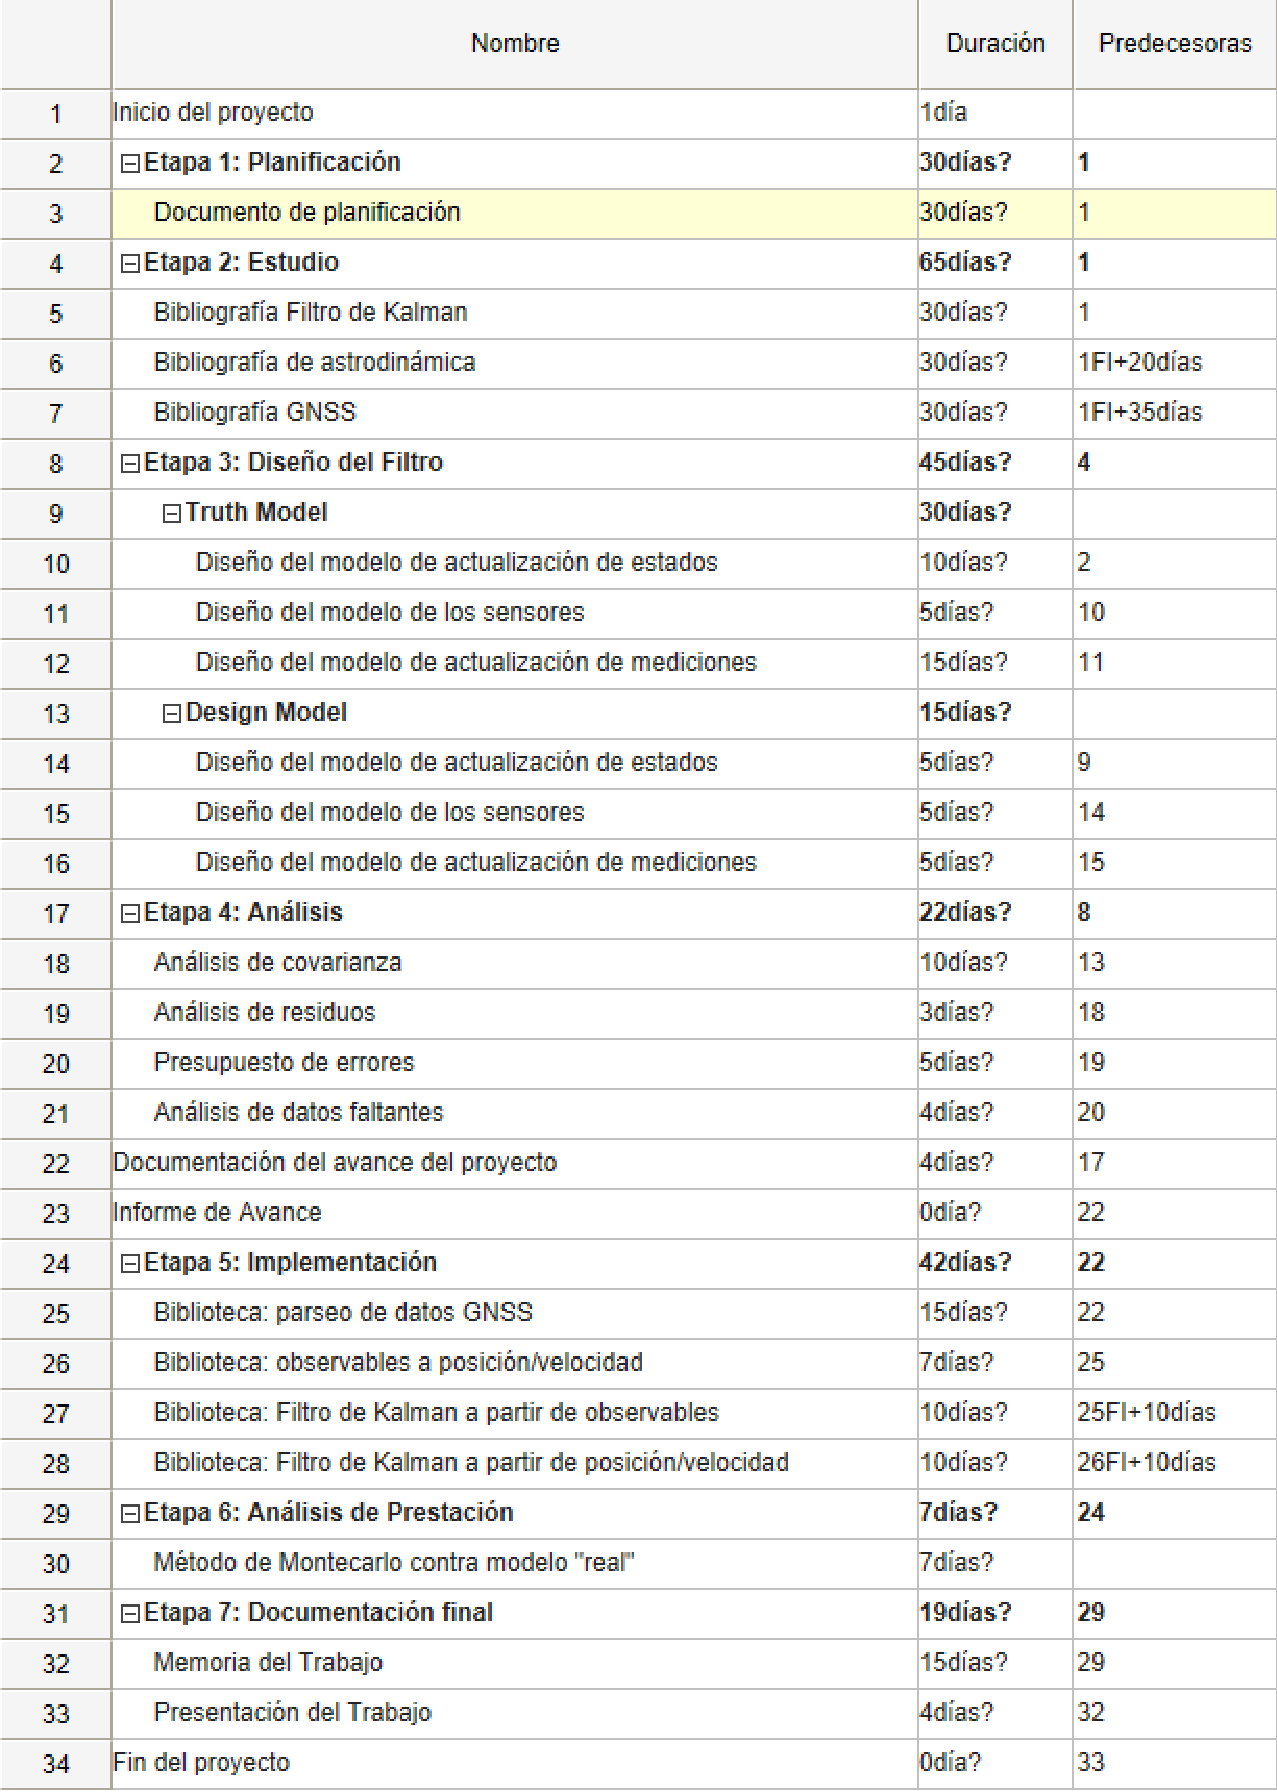
\includegraphics[width=.7\textwidth]{./Figuras/WBS.pdf}
\caption{Desgloce de tareas}
\label{fig:wbs}
\end{figure}

\vspace{25px}

\section{7. Diagrama de Activity On Node}
\label{sec:AoN}

\begin{figure}[H]
\centering 
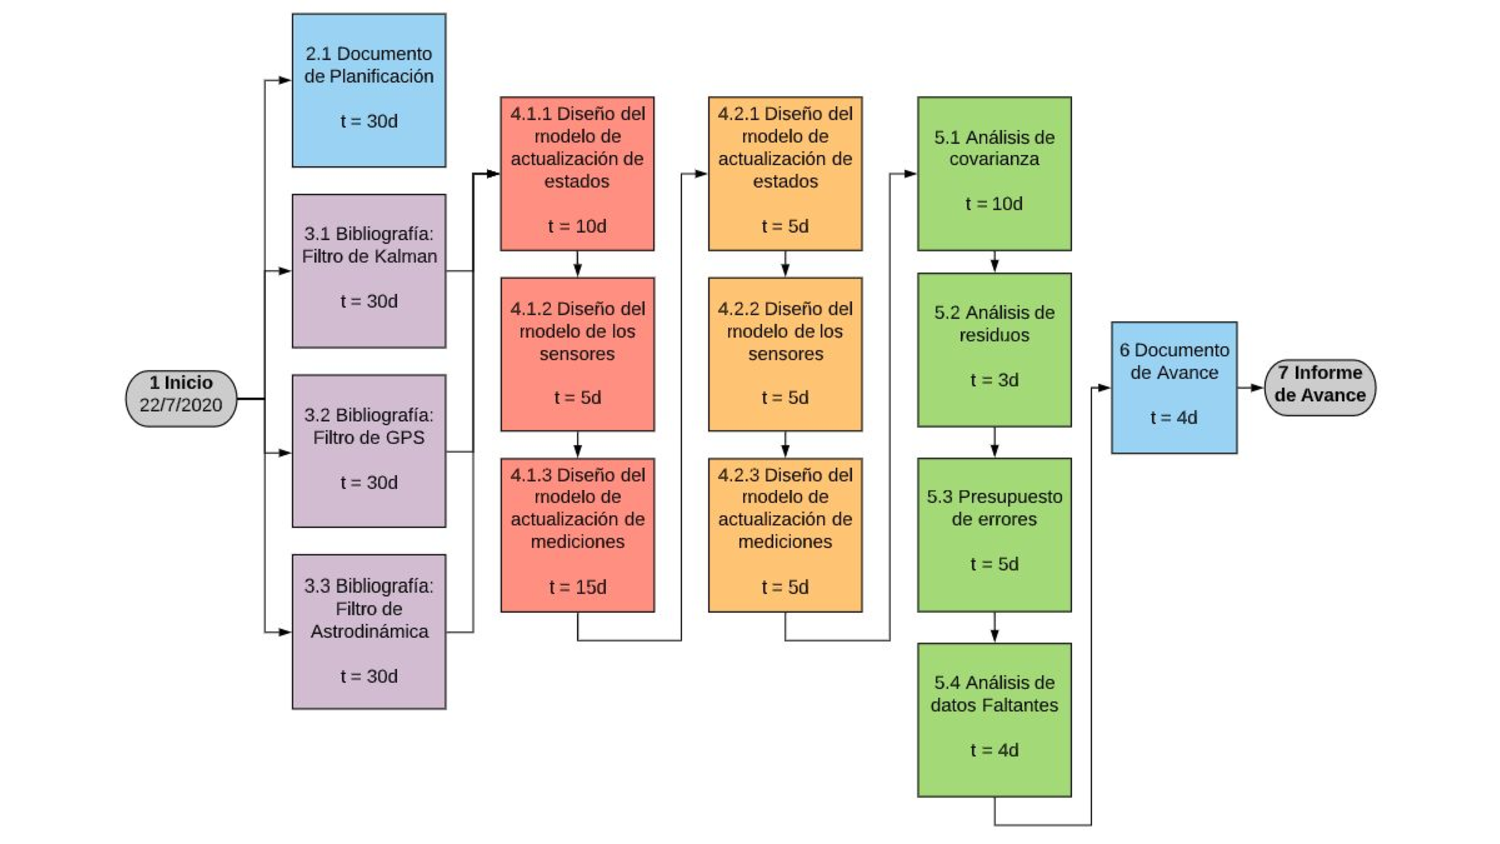
\includegraphics[page=1, width=\textwidth]{./Figuras/AoN.pdf}
\caption{Diagrama en \textit{Activity on Node} (Primera parte)}
\label{fig:AoN}
\end{figure}

\begin{figure}[H]
\centering 
\includegraphics[page=2, width=\textwidth]{./Figuras/AoN.pdf}
\caption{Diagrama en \textit{Activity on Node} (Segunda parte)}
\label{fig:AoN}
\end{figure}


\section{8. Diagrama de Gantt}
\label{sec:gantt}

\begin{figure}[H]
\centering 
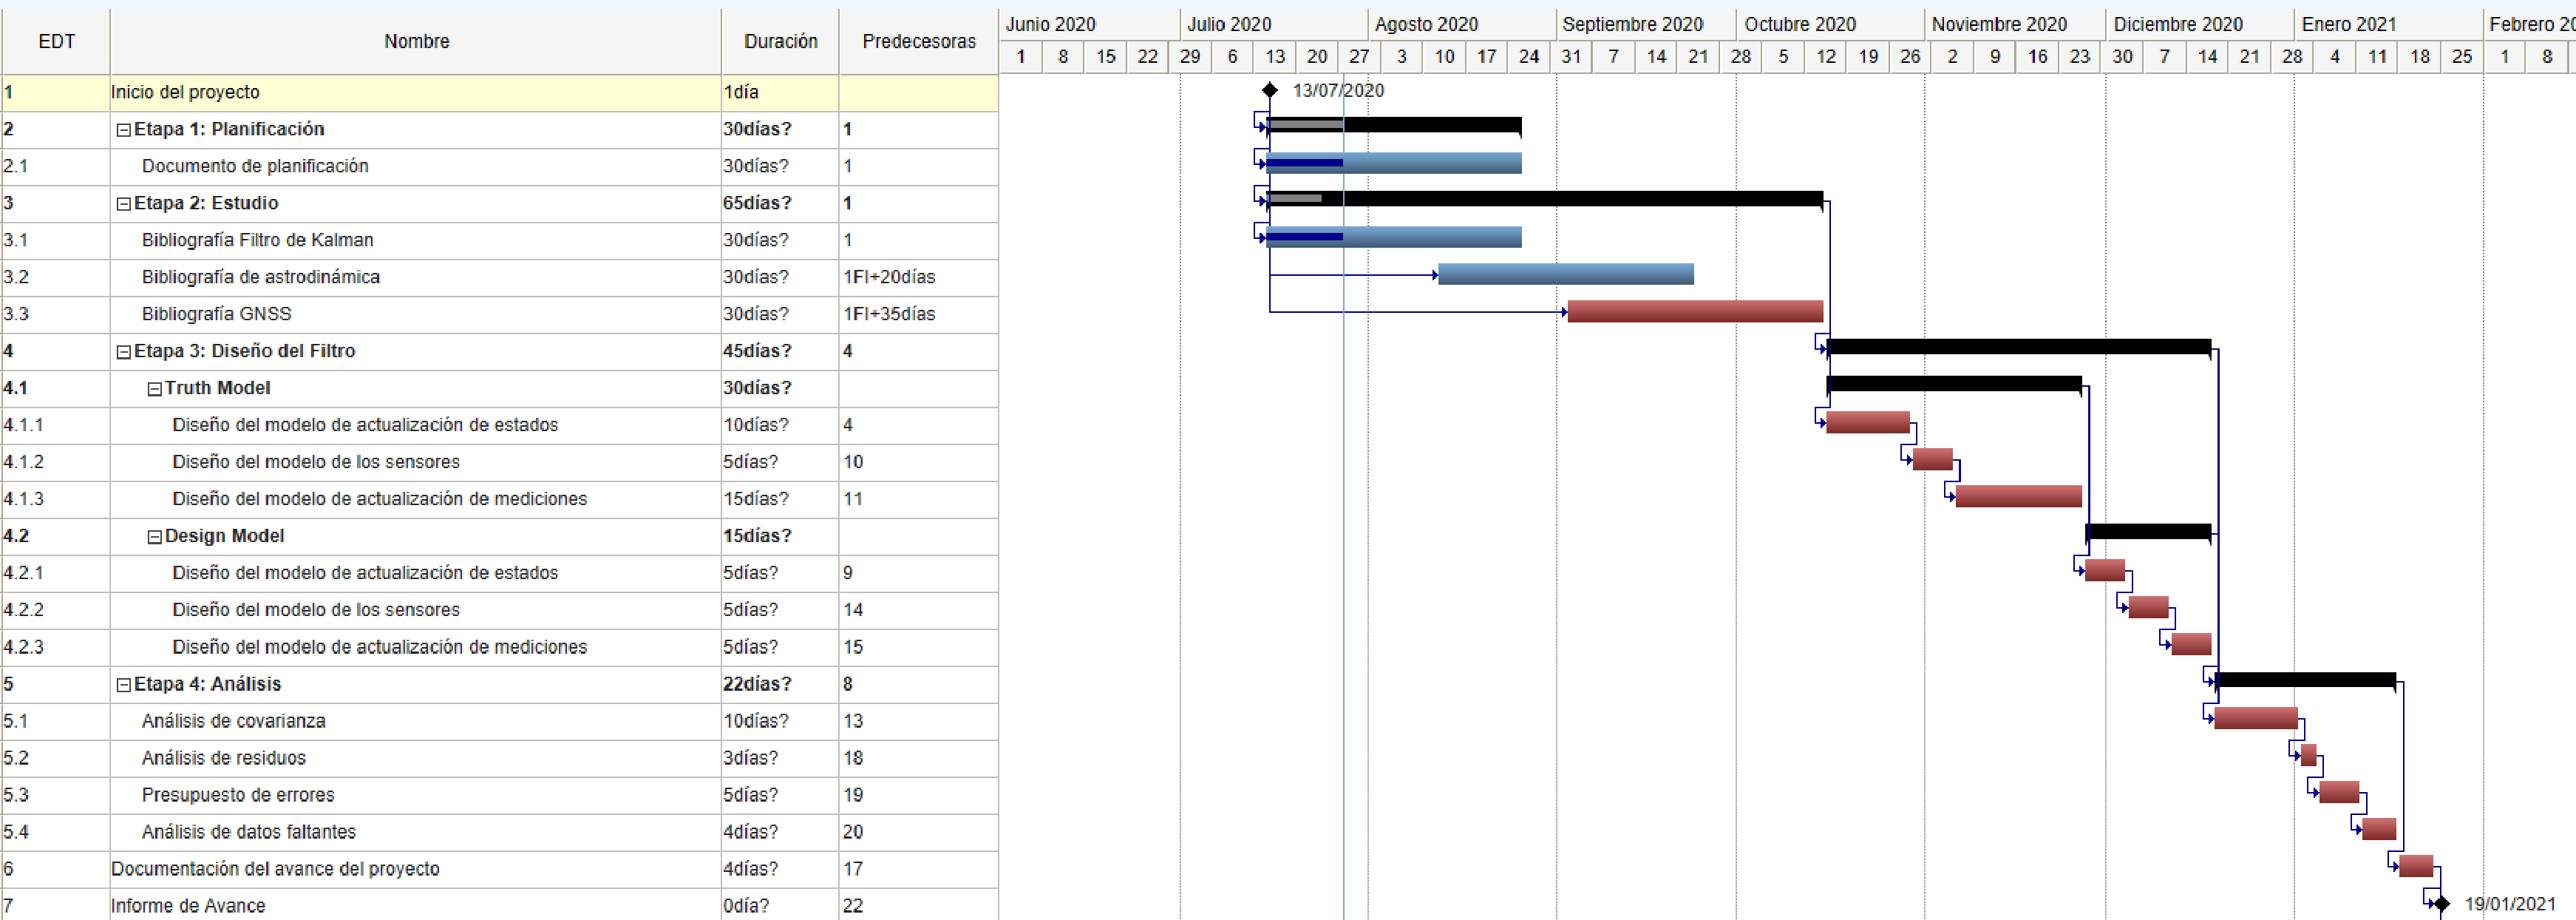
\includegraphics[width=1.4\textwidth, angle =90]{./Figuras/Gantt1.pdf}
\caption{Diagrama de Gantt (primera parte)}
\label{fig:Gantt}
\end{figure}

\begin{figure}[H]
\centering 
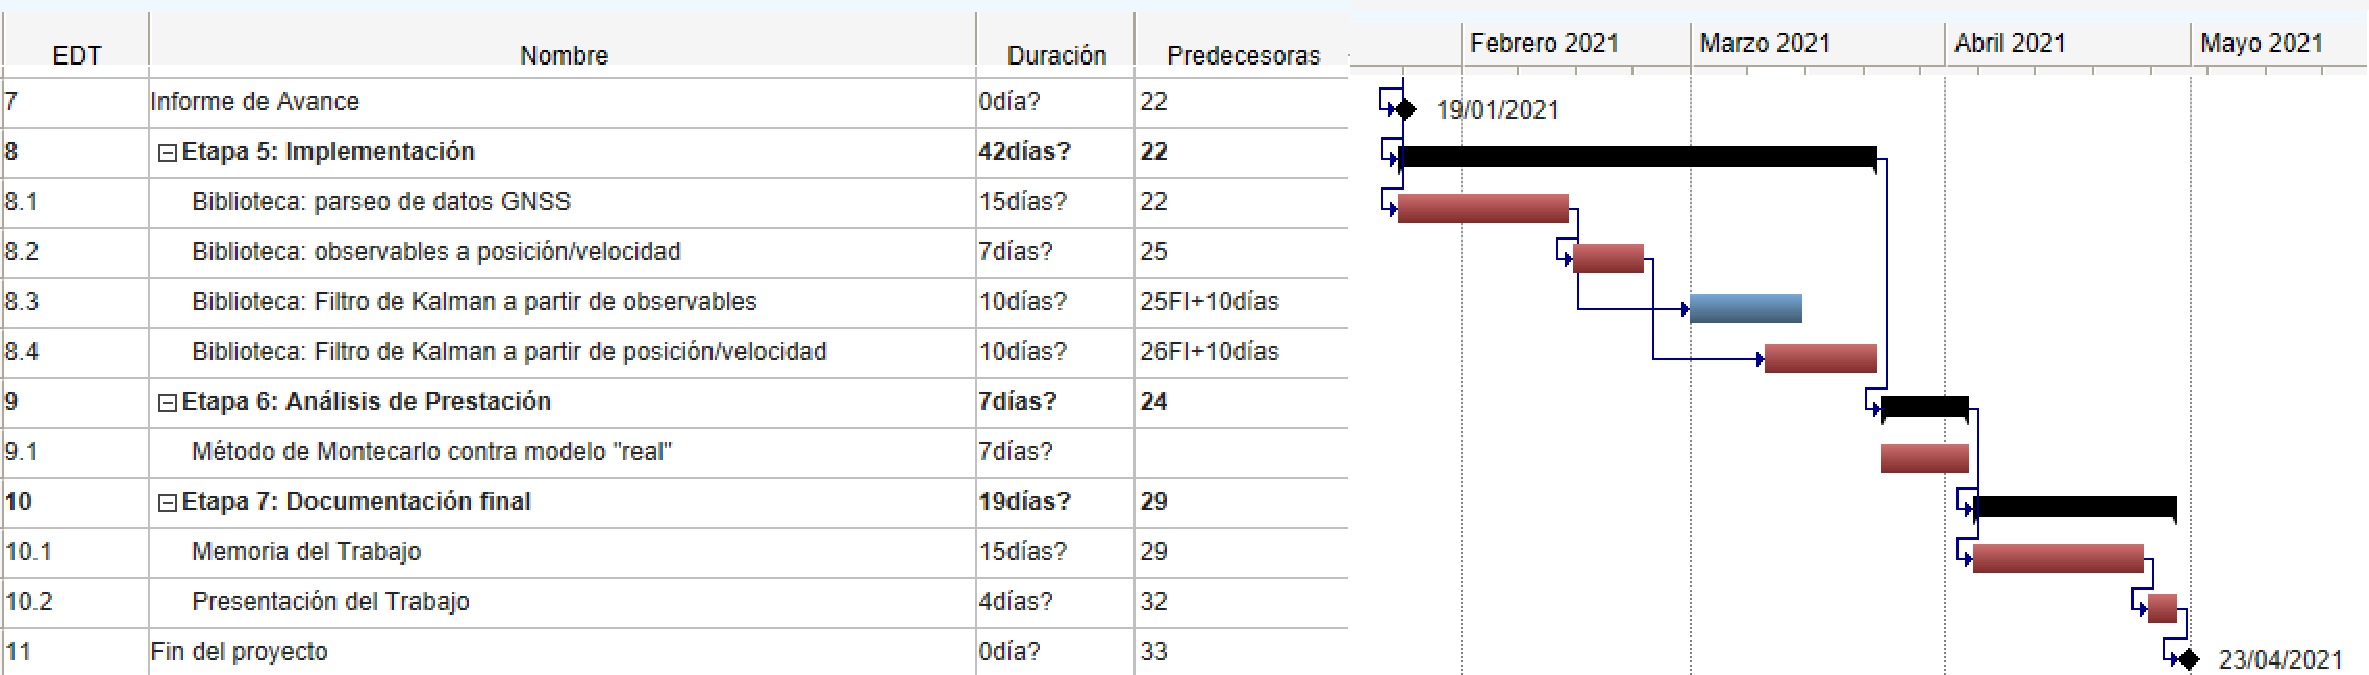
\includegraphics[width=\textwidth]{./Figuras/Gantt2.pdf}
\caption{Diagrama de Gantt (segunda parte)}
\label{fig:Gantt}
\end{figure}


\section{9. Matriz de uso de recursos de materiales}
\label{sec:recursos}

\begin{table}[H]
\label{tab:recursos}
\centering
\begin{tabularx}{\linewidth}{@{}|c|X|>{\centering}m{2cm}|c|c|@{}}
\hline
\cellcolor[HTML]{C0C0C0} & \cellcolor[HTML]{C0C0C0} & \multicolumn{3}{c|}{\cellcolor[HTML]{C0C0C0}Recursos requeridos (días)} \\ \cline{3-5} 
\multirow{-2}{*}{\cellcolor[HTML]{C0C0C0}\begin{tabular}[c]{@{}c@{}}Código\\ WBS\end{tabular}} & \multirow{-2}{*}{\cellcolor[HTML]{C0C0C0}\begin{tabular}[c]{@{}c@{}}Nombre \\ Tarea\end{tabular}} & Procesador de texto & Matlab & EDU-CIAA \\ \hline
\rowcolor{lightgray!50}
\textbf{1}	& \textbf{Inicio del proyecto}  					& \textbf{0} 	& \textbf{0} 		& \textbf{0} \\ \hline
\rowcolor{lightgray!50}
\textbf{2}	& \textbf{Etapa 1: Planificación} 						& \textbf{30} 	& \textbf{0} 	& \textbf{0} \\ \hline
2.1 		& Documento de planificación 							& 30 			&  				& 	\\ \hline
\rowcolor{lightgray!50}
\textbf{3}	& \textbf{Etapa 2: Estudio} 							& \textbf{65} 	& \textbf{0}	& \textbf{0} \\ \hline
3.1			& Bibliografía Filtro de Kalman						& 30 			&  				& 	\\ \hline
3.2			& Bibliografía Astrodinámica							& 30 			&  				& 	\\ \hline
3.3			& Bibliografía GNSS										& 30 			&  				& 	\\ \hline
\rowcolor{lightgray!50}
\textbf{4}	& \textbf{Etapa 3: Diseño del Filtro}					& \textbf{0}	& \textbf{45}	& \textbf{0} \\ \hline
\rowcolor{lightgray!25}
4.1			& Truth model											& 0	 			& 30 			& 0 \\ \hline
4.1.1		& Diseño del modelo de actualización de estados		& 	 			& 10 			& 	\\ \hline
4.1.2		& Diseño del modelo de los sensores 					& 	 			& 5 			& 	\\ \hline
4.1.3		& Diseño del modelo de actualización de mediciones	& 	 			& 10 			& 	\\ \hline
\rowcolor{lightgray!25}
4.2			& Design model											& 0 			& 15 			& 0 \\ \hline
4.2.1		& Diseño del modelo de actualización de estados		& 	 			& 5 			&   \\ \hline
4.2.2		& Diseño del modelo de los sensores 					& 	 			& 5 			& 	\\ \hline
4.2.3		& Diseño del modelo de actualización de mediciones	& 	 			& 5 			& 	\\ \hline
\rowcolor{lightgray!50}
\textbf{5}	& \textbf{Etapa 4: Análisis}							& \textbf{0}	& \textbf{22}	& \textbf{0} \\ \hline
5.1			& Análisis de covarianza								& 	 			& 10 			& 	\\ \hline
5.2			& Análisis de residuos 									& 	 			& 3 			& 	\\ \hline
5.3			& Presupuesto de errores								& 	 			& 5 			& 	\\ \hline
5.4			& Análisis de datos faltantes							& 	 			& 4 			& 	\\ \hline
\rowcolor{lightgray!50}
\textbf{6}	& \textbf{Documentación del avance del proyecto} 		& \textbf{4}	& \textbf{0}	& \textbf{0} \\ \hline
\rowcolor{lightgray!50}
\textbf{7} 	& \textbf{Informe de avance} 							& \textbf{0} 	& \textbf{0}	& \textbf{0} \\ \hline
\rowcolor{lightgray!50}
\textbf{8}	& \textbf{Etapa 5: Implementación}						& \textbf{0} 	& \textbf{0} 	& \textbf{42}\\ \hline
8.1			& Biblioteca: parseo de datos GNSS						& 	 			& 	 			& 15\\ \hline
8.2			& Biblioteca: observables a pos/vel					& 	 			& 	 			& 7 \\ \hline
8.3			& Biblioteca: Filtro de Kalman a partir de observable & 	 			& 	 			& 10\\ \hline
8.4			& Biblioteca: Filtro de Kalman a partir de pos/vel 	& 	 			& 	 			& 10\\ \hline
\rowcolor{lightgray!50}
\textbf{9} 	& \textbf{Etapa 6: Análisis de prestación}				& \textbf{0}	& \textbf{7} 	& \textbf{7} \\ \hline
9.1			& Metodo de Montecarlo contra modelo 'real' 			& 	 			& 7 			& 7 \\ \hline
\rowcolor{lightgray!50}
\textbf{10}	& \textbf{Etapa 7: Documentación final}				& \textbf{19} 	& \textbf{0} 	& \textbf{0} \\ \hline
10.1 		& Memoria del trabajo		 							& 15 			& 	 			& 	\\ \hline
10.2 		& Presentación del trabajo		 						& 4 			& 	 			& 	\\ \hline
\rowcolor{lightgray!50}
\textbf{11}	& \textbf{Fin del proyecto} 							& \textbf{0} 	& \textbf{0}	& \textbf{0} \\ \hline
\end{tabularx}%
\end{table}


\section{10. Presupuesto detallado del proyecto}
\label{sec:presupuesto}

\begin{table}[H]
\centering
\begin{tabularx}{\linewidth}{@{}|X|c|r|r|@{}}
\hline
\rowcolor[HTML]{C0C0C0} 
\multicolumn{4}{|c|}{\cellcolor[HTML]{C0C0C0}COSTOS DIRECTOS} \\ \hline
\rowcolor[HTML]{C0C0C0} 
Descripción &
  \multicolumn{1}{c|}{\cellcolor[HTML]{C0C0C0}Cantidad} &
  \multicolumn{1}{c|}{\cellcolor[HTML]{C0C0C0}Costo unitario (Pesos)} &
  \multicolumn{1}{c|}{\cellcolor[HTML]{C0C0C0}Valor total (Pesos)} \\ \hline
Horas Hombre & 
  \multicolumn{1}{c|}{600} &  
  \multicolumn{1}{c|}{a definir} &  
  \multicolumn{1}{c|}{a definir}  \\ \hline
\multicolumn{3}{|c|}{SUBTOTAL} &
  \multicolumn{1}{c|}{a definr} \\ \hline
\rowcolor[HTML]{C0C0C0} 
\multicolumn{4}{|c|}{\cellcolor[HTML]{C0C0C0}COSTOS INDIRECTOS} \\ \hline
\rowcolor[HTML]{C0C0C0} 
Descripción &
  \multicolumn{1}{c|}{\cellcolor[HTML]{C0C0C0}Cantidad} &
  \multicolumn{1}{c|}{\cellcolor[HTML]{C0C0C0}Valor unitario} &
  \multicolumn{1}{c|}{\cellcolor[HTML]{C0C0C0}Valor total} \\ \hline
\multicolumn{1}{|l|}{EDU-CIAA} &
  \multicolumn{1}{c|}{1} &  
  \multicolumn{1}{c|}{5000} &  
  \multicolumn{1}{c|}{5000}  \\ \hline    
\multicolumn{3}{|c|}{SUBTOTAL} &
  \multicolumn{1}{c|}{5000} \\ \hline
\rowcolor[HTML]{C0C0C0}
\multicolumn{3}{|c|}{TOTAL} &
  \multicolumn{1}{c|}{a definr} \\ \hline
\end{tabularx}%
\end{table}


\section{11. Matriz de asignación de responsabilidades}
\label{sec:responsabilidades}

\begin{table}[htpb]
\centering
\resizebox{\textwidth}{!}{%
\begin{tabular}{|c|c|m{3cm}|m{3cm}|m{3cm}|}
\hline
\rowcolor[HTML]{C0C0C0} 
\cellcolor[HTML]{C0C0C0} &
  \cellcolor[HTML]{C0C0C0} &
  \multicolumn{3}{c|}{\cellcolor[HTML]{C0C0C0}} \\ \cline{3-5} 
\rowcolor[HTML]{C0C0C0} 
\cellcolor[HTML]{C0C0C0} &
  \cellcolor[HTML]{C0C0C0} &
  Responsable &
  Orientador &
  Cliente \\ \cline{3-5} 
\rowcolor[HTML]{C0C0C0} 
\multirow{-3}{*}{\cellcolor[HTML]{C0C0C0}\begin{tabular}[c]{@{}c@{}}Código\\ WBS\end{tabular}} &
  \multirow{-3}{*}{\cellcolor[HTML]{C0C0C0}Nombre de la tarea} &
	\authorname &
  	\supname &
  	\clientename \\ \hline

\rowcolor{lightgray!50}
\textbf{1}	& \textbf{Inicio del proyecto}  						& 			 	& 			 	&  \\ \hline
\rowcolor{lightgray!50}
\textbf{2}	& \textbf{Etapa 1: Planificación} 						& 			 	& 				&			 \\ \hline
2.1 		& Documento de planificación 							& P 			& I				& A	\\ \hline
\rowcolor{lightgray!50}
\textbf{3}	& \textbf{Etapa 2: Estudio} 							& 			 	& 				&  \\ \hline
3.1			& Bibliografía Filtro de Kalman						& P 			& A 			& C	\\ \hline
3.2			& Bibliografía Astrodinámica							& P 			& A				& C	\\ \hline
3.3			& Bibliografía GNSS										& P 			& A				& C	\\ \hline
\rowcolor{lightgray!50}
\textbf{4}	& \textbf{Etapa 3: Diseño del Filtro}					& 				& 				& 	 \\ \hline
\rowcolor{lightgray!25}
4.1			& Truth model											& 	 			& 	 			&  \\ \hline
4.1.1		& Diseño del modelo de actualización de estados		& P	 			& C/A 			& I	\\ \hline
4.1.2		& Diseño del modelo de los sensores 					& P	 			& C/A 			& I	\\ \hline
4.1.3		& Diseño del modelo de actualización de mediciones	& P	 			& C/A			& I	\\ \hline
\rowcolor{lightgray!25}
4.2			& Design model											& 	 			& 	 			& 	\\ \hline
4.2.1		& Diseño del modelo de actualización de estados		& P	 			& C 			& A  \\ \hline
4.2.2		& Diseño del modelo de los sensores 					& P	 			& C 			& A	\\ \hline
4.2.3		& Diseño del modelo de actualización de mediciones	& P	 			& C	 			& A	\\ \hline
\rowcolor{lightgray!50}
\textbf{5}	& \textbf{Etapa 4: Análisis}							& 				& 				&  \\ \hline
5.1			& Análisis de covarianza								& P	 			& C	 			& A	\\ \hline
5.2			& Análisis de residuos 									& P	 			& C	 			& A	\\ \hline
5.3			& Presupuesto de errores								& P 			& C	 			& A	\\ \hline
5.4			& Análisis de datos faltantes							& P 			& C	 			& A	\\ \hline
\rowcolor{lightgray!50}
\textbf{6}	& \textbf{Documentación del avance del proyecto} 		& P				& I				& A \\ \hline
\rowcolor{lightgray!50}
\textbf{7} 	& \textbf{Informe de avance} 							& 			 	& 				&  \\ \hline
\rowcolor{lightgray!50}
\textbf{8}	& \textbf{Etapa 5: Implementación}						& 			 	& 			 	& \\ \hline
8.1			& Biblioteca: parseo de datos GNSS						& P	 			& C	 			& C/A \\ \hline
8.2			& Biblioteca: observables a pos/vel					& P	 			& C	 			& A	\\ \hline
8.3			& Biblioteca: Filtro de Kalman a partir de observable & P	 			& C	 			& A	\\ \hline
8.4			& Biblioteca: Filtro de Kalman a partir de pos/vel 	& P	 			& C	 			& A	\\ \hline
\rowcolor{lightgray!50}
\textbf{9} 	& \textbf{Etapa 6: Análisis de prestación}				& 				& 			 	&  \\ \hline
9.1			& Metodo de Montecarlo contra modelo 'real' 			& P	 			& C  			& A \\ \hline
\rowcolor{lightgray!50}
\textbf{10}	& \textbf{Etapa 7: Documentación final}				& 			 	& 			 	&  \\ \hline
10.1 		& Memoria del trabajo		 							& P 			& A	 			& A	\\ \hline
10.2 		& Presentación del trabajo		 						& P 			& I	 			& I	\\ \hline
\rowcolor{lightgray!50}
\textbf{11}	& \textbf{Fin del proyecto} 							& 			 	& 				& \\ \hline
\end{tabular}%
}
\end{table}

{\footnotesize
Referencias:
\begin{itemize}
	\item P = Responsabilidad Primaria
	\item S = Responsabilidad Secundaria
	\item A = Aprobación
	\item I = Informado
	\item C = Consultado
\end{itemize}
} %footnotesize

\section{12. Gestión de riesgos}
\label{sec:riesgos}

\begin{consigna}{red}
a) Identificación de los riesgos (al menos cinco) y estimación de sus consecuencias:
 
Riesgo 1: detallar el riesgo (riesgo es algo que si ocurre altera los planes previstos)
\begin{itemize}
\item Severidad (S): mientras más severo, más alto es el número (usar números del 1 al 10).\\
Justificar el motivo por el cual se asigna determinado número de severidad (S).
\item Probabilidad de ocurrencia (O): mientras más probable, más alto es el número (usar del 1 al 10).\\
Justificar el motivo por el cual se asigna determinado número de (O). 
\end{itemize}   

Riesgo 2:
\begin{itemize}
\item Severidad (S): 
\item Ocurrencia (O):
\end{itemize}

Riesgo 3:
\begin{itemize}
\item Severidad (S): 
\item Ocurrencia (O):
\end{itemize}


b) Tabla de gestión de riesgos:      (El RPN se calcula como RPN=SxO)

\begin{table}[htpb]
\centering
\begin{tabularx}{\linewidth}{@{}|X|c|c|c|c|c|c|@{}}
\hline
\rowcolor[HTML]{C0C0C0} 
Riesgo & S & O & RPN & S* & O* & RPN* \\ \hline
       &   &   &     &    &    &      \\ \hline
       &   &   &     &    &    &      \\ \hline
       &   &   &     &    &    &      \\ \hline
       &   &   &     &    &    &      \\ \hline
       &   &   &     &    &    &      \\ \hline
\end{tabularx}%
\end{table}

Criterio adoptado: 
Se tomarán medidas de mitigación en los riesgos cuyos números de RPN sean mayores a ....

Nota: los valores marcados con (*) en la tabla corresponden luego de haber aplicado la mitigación.

c) Plan de mitigación de los riesgos que originalmente excedían el RPN máximo establecido:
 
Riesgo 1: Plan de mitigación (si por el RPN fuera necesario elaborar un plan de mitigación).
  Nueva asignación de S y O, con su respectiva justificación:
  - Severidad (S): mientras más severo, más alto es el número (usar números del 1 al 10).
          Justificar el motivo por el cual se asigna determinado número de severidad (S).
  - Probabilidad de ocurrencia (O): mientras más probable, más alto es el número (usar del 1 al 10).
          Justificar el motivo por el cual se asigna determinado número de (O).

Riesgo 2: Plan de mitigación (si por el RPN fuera necesario elaborar un plan de mitigación).
 
Riesgo 3: Plan de mitigación (si por el RPN fuera necesario elaborar un plan de mitigación)

\end{consigna}


\section{13. Gestión de la calidad}
\label{sec:calidad}

\begin{consigna}{red}
Para cada uno de los requerimientos del proyecto indique:
\begin{itemize} 
\item Req \#1: Copiar acá el requerimiento.

Verificación y validación:

\begin{itemize}
\item Verificación para confirmar si se cumplió con lo requerido antes de mostrar el sistema al cliente:\\
Detallar 
\item Validación con el cliente para confirmar que está de acuerdo en que se cumplió con lo requerido:\\
Detallar  
\end{itemize}

\end{itemize}

Tener en cuenta que en este contexto se pueden mencionar simulaciones, cálculos, revisión de hojas de datos, consulta con expertos, etc.

\end{consigna}

\section{14. Comunicación del proyecto}
\label{sec:comunicaciones}

\begin{consigna}{red}
El plan de comunicación del proyecto es el siguiente:
\end{consigna}

% Please add the following required packages to your document preamble:
% \usepackage{graphicx}
% \usepackage[table,xcdraw]{xcolor}
% If you use beamer only pass "xcolor=table" option, i.e. \documentclass[xcolor=table]{beamer}
\begin{table}[htpb]
\centering
\resizebox{\textwidth}{!}{%
\begin{tabular}{|c|c|c|c|c|c|}
\hline
\rowcolor[HTML]{C0C0C0} 
\multicolumn{6}{|c|}{\cellcolor[HTML]{C0C0C0}PLAN DE COMUNICACIÓN DEL PROYECTO}           \\ \hline
\rowcolor[HTML]{C0C0C0} 
¿Qué comunicar? & Audiencia & Propósito & Frecuencia & Método de comunicac. & Responsable \\ \hline
                &           &           &            &                      &             \\ \hline
                &           &           &            &                      &             \\ \hline
                &           &           &            &                      &             \\ \hline
                &           &           &            &                      &             \\ \hline
                &           &           &            &                      &             \\ \hline
\end{tabular}%
}
\end{table}

\section{15. Gestión de Compras}
\label{sec:compras}

\begin{consigna}{red}
En caso de tener que comprar elementos o contratar servicios:
a) Explique con qué criterios elegiría a un proveedor.
b) Redacte el Statement of Work correspondiente.
\end{consigna}

\section{16. Seguimiento y control}
\label{sec:seguimiento}

\begin{consigna}{red}
Para cada tarea del proyecto establecer la frecuencia y los indicadores con los se seguirá su avance y quién será el responsable de hacer dicho seguimiento y a quién debe comunicarse la situación (en concordancia con el Plan de Comunicación del proyecto).

El indicador de avance tiene que ser algo medible, mejor incluso si se puede medir en \% de avance. Por ejemplo,se pueden indicar en esta columna cosas como ``cantidad de conexiones ruteadeas'' o ``cantidad de funciones implementadas'', pero no algo genérico y ambiguo como ``\%'', porque el lector no sabe porcentaje de qué cosa.

\end{consigna}

\begin{table}[!htpb]
\centering
\begin{tabularx}{\linewidth}{@{}|X|X|X|X|X|X|@{}}
\hline
\rowcolor[HTML]{C0C0C0} 
\multicolumn{6}{|c|}{\cellcolor[HTML]{C0C0C0}SEGUIMIENTO DE AVANCE}                                                                       \\ \hline
\rowcolor[HTML]{C0C0C0} 
Tarea del WBS & Indicador de avance & Frecuencia de reporte & Resp. de seguimiento & Persona a ser informada & Método de comunic. \\ \hline
 &  &  &  &  &  \\ \hline
 &  &  &  &  &  \\ \hline
 &  &  &  &  &  \\ \hline
 &  &  &  &  &  \\ \hline
 &  &  &  &  &  \\ \hline
\end{tabularx}%
%}
\end{table}

\section{17. Procesos de cierre}    
\label{sec:cierre}

\begin{consigna}{red}
Establecer las pautas de trabajo para realizar una reunión final de evaluación del proyecto, tal que contemple las siguientes actividades:

\begin{itemize}
\item Pautas de trabajo que se seguirán para analizar si se respetó el Plan de Proyecto original:
 - Indicar quién se ocupará de hacer esto y cuál será el procedimiento a aplicar. 
\item Identificación de las técnicas y procedimientos útiles e inútiles que se utilizaron, y los problemas que surgieron y cómo se solucionaron:
 - Indicar quién se ocupará de hacer esto y cuál será el procedimiento para dejar registro.
\item Indicar quién organizará el acto de agradecimiento a todos los interesados, y en especial al equipo de trabajo y colaboradores:
  - Indicar esto y quién financiará los gastos correspondientes.
\end{itemize}

\end{consigna}


\end{document}
